\documentclass[10pt]{article}

% ----- Page geometry: NeurIPS-style single-column.
\usepackage[letterpaper, total={5.5in, 9in}, top=1.0in, left=1.5in]{geometry}

% ----- Standard packages.
\usepackage[utf8]{inputenc}
\usepackage[T1]{fontenc}
\usepackage{microtype}
\usepackage{amsmath, amssymb, amsthm, mathtools}
\usepackage{graphicx}
\usepackage{booktabs}
\usepackage{caption}
\usepackage{subcaption}
\usepackage{hyperref}
\usepackage{url}
\usepackage{xcolor}
\usepackage{natbib}

% ----- Title formatting.
\usepackage{titlesec}
\titleformat{\section}{\normalfont\large\bfseries}{\thesection}{1em}{}
\titleformat{\subsection}{\normalfont\normalsize\bfseries}{\thesubsection}{1em}{}

% ----- Theorem-like environments.
\newtheorem{proposition}{Proposition}
\newtheorem{remark}{Remark}

% ----- Math shortcuts used throughout.
\newcommand{\R}{\mathbb{R}}
\newcommand{\Z}{\mathbb{Z}}
\newcommand{\E}{\mathbb{E}}
\DeclareMathOperator{\softmax}{softmax}
\DeclareMathOperator{\Tr}{Tr}

% ----- Paper title and author block.
\title{\textbf{Multi-task grokking on modular arithmetic:\\
do shared Fourier features emerge?}}
\author{Zaidan Mir\thanks{Department of Computer Science, Kingston University.
Code and figures: \url{https://github.com/zaidanmir/grokking-multitask}.
Correspondence: \texttt{zaidan2440@gmail.com}.}}
\date{}

% ----- Hyperref colours.
\hypersetup{colorlinks=true, linkcolor=black, citecolor=blue!60!black,
            urlcolor=blue!60!black, pdftitle={Multi-task grokking on modular arithmetic}}

\begin{document}

\maketitle

\begin{center}
\textit{Preprint. Under review.}
\end{center}

\begin{abstract}
\noindent
Grokking is the phenomenon in which a small neural network trained on a
synthetic algorithmic task first memorises the training set and then,
after thousands of additional training steps with no apparent progress,
abruptly generalises. \citet{nanda2023progress} showed that during the
apparent plateau a one-layer transformer is silently constructing a
discrete-Fourier-transform algorithm for modular addition. We extend
that analysis to a \emph{multi-task} setting in which a single one-layer
transformer is trained jointly on three modular arithmetic tasks ---
addition, subtraction, and multiplication modulo a prime $p$. Two of
these tasks live on the additive group $\Z/p\Z$ and one lives on the
multiplicative group $(\Z/p\Z)^*$, which has different Fourier-transform
structure.

We replicate the single-task addition baseline of
\citet{nanda2023progress} ($p = 113$, $\mathrm{train\_frac} = 0.30$,
AdamW with $\mathrm{weight\_decay} = 1.0$, grokking at step
$\sim$$7{,}200$) and obtain analogous sharp grokking transitions for
single-task subtraction and multiplication. Joint training on
\textsc{add}+\textsc{sub} grokes \emph{faster} than either single-task
baseline, suggesting that the shared additive Fourier basis is
discovered more quickly under joint gradient pressure. Joint training on
\textsc{add}+\textsc{sub}+\textsc{mul} produces a qualitatively
different dynamic: instead of a sharp plateau-then-collapse transition,
test accuracy on each task rises smoothly through 75{,}000 training
steps, reaching $0.60 / 0.48 / 0.32$ on the three tasks but never
crossing the 0.95 grok threshold. We argue this slow-ramp dynamic
reflects a residual-stream capacity competition between the two
distinct Fourier circuits that the additive and multiplicative tasks
each require. Code, configs, checkpoints, and all per-step metric
histories are released for reproducibility and continued analysis.
\end{abstract}


\section{Introduction}
\label{sec:intro}

Train a small transformer on $(a + b) \bmod p$ for a prime $p$, with a
hard 30/70 train/test split and aggressive weight decay. The training loss
collapses within a few hundred gradient steps, so the network has memorised
the training set. The test loss does not move. After tens of thousands of
\emph{additional} steps with no apparent progress, the test loss abruptly
collapses and the model generalises. \citet{power2022grokking} named this
phenomenon \emph{grokking} and showed that it occurs across a family of
small algorithmic tasks. \citet{nanda2023progress} subsequently showed
that during the apparent plateau the network is silently constructing a
discrete-Fourier-transform algorithm for the underlying group operation,
and that weight-decay-driven implicit regularisation is what tips the
optimiser from memorising circuits to generalising circuits.

Grokking sits at the intersection of three research frontiers:
generalisation theory, mechanistic interpretability, and optimisation
dynamics. The single-task setting is now reasonably well understood. The
\emph{multi-task} setting is not.

\paragraph{This paper.} We ask three questions:
\begin{enumerate}
\item When a single one-layer transformer is trained jointly on
      $\{+, -, \times\} \bmod p$, does grokking still occur on each task?
\item Does multi-task training accelerate, delay, or qualitatively change
      the per-task grokking dynamics relative to single-task training?
\item Are the discovered Fourier features shared across tasks or
      task-specific? In particular, do addition and subtraction (which
      both live on the additive group $\Z/p\Z$) develop a shared feature
      set, and does multiplication (which lives on the multiplicative
      group $(\Z/p\Z)^*$) develop a separate basis?
\end{enumerate}

\paragraph{Why these questions.}
All three operations have closed-form Fourier solutions (Section
\ref{sec:background}), so we can make falsifiable predictions about which
features should emerge. The multiplicative group $(\Z/p\Z)^*$ is cyclic of
order $p - 1$, which is a different cyclic group from the additive
$\Z/p\Z$ of order $p$, so the two groups have non-overlapping Fourier
bases. A single residual stream that solves all three tasks must therefore
either reuse one basis for both groups or carve out task-specific
sub-spaces. Both possibilities are interesting: the first would suggest
the model has discovered a representation that abstracts over group
structure, the second would suggest the model is internally
``time-multiplexing'' between two algorithms.

\paragraph{Contributions.}
\begin{itemize}
\item A clean replication of the \citet{nanda2023progress} single-task
      addition baseline at the published hyperparameters
      ($p = 113$, $\mathrm{train\_frac} = 0.30$, AdamW with
      $\mathrm{weight\_decay} = 1.0$).
\item A characterisation of per-task grokking dynamics in joint training
      on add+subtract and on add+subtract+multiply, with three random
      seeds for robustness.
\item A Fourier-feature analysis of the multi-task model's embedding
      matrix, comparing additive-group and multiplicative-group
      decompositions and quantifying overlap with the corresponding
      single-task models via cosine similarity.
\item Per-head ablations showing that attention heads partially
      specialise toward operation-conditional features.
\item A fully reproducible code release with config files, per-step
      metric histories, and all figures.\footnote{%
      \url{https://github.com/zaidanmir/grokking-multitask}}
\end{itemize}

The rest of the paper is structured as follows. Section
\ref{sec:background} reviews the algebraic and Fourier prerequisites and
the published single-task grokking story. Section \ref{sec:methods}
describes the model architecture, optimiser, and dataset construction.
Section \ref{sec:replication} reports the single-task replication.
Section \ref{sec:multitask} reports the multi-task experiments. Section
\ref{sec:analysis} reports the mechanistic Fourier analysis and head
ablations. Section \ref{sec:discussion} discusses what the findings imply
about transformer representations, and Section \ref{sec:future_work}
sketches open follow-ups.


\section{Background}
\label{sec:background}

\subsection{Modular arithmetic as a group-theoretic task}

Let $p$ be an odd prime and let $\Z/p\Z = \{0, 1, \ldots, p-1\}$.
Under addition modulo $p$, $\Z/p\Z$ is a cyclic group of order $p$.
Under multiplication modulo $p$, the non-zero residues
$(\Z/p\Z)^* = \{1, 2, \ldots, p-1\}$ form a cyclic group of order $p - 1$
generated by some primitive root $g$. The additive and multiplicative
groups are both cyclic, but they have \emph{different} order, so their
Fourier bases live on different index sets.

\subsection{The discrete Fourier transform on $\Z/p\Z$}

For a function $f : \Z/p\Z \to \R$, the discrete Fourier transform (DFT) is
\begin{equation}
\hat f(k)
= \frac{1}{p} \sum_{n = 0}^{p - 1} f(n) \, e^{-2 \pi i k n / p}
\qquad k = 0, 1, \ldots, p - 1.
\label{eq:dft}
\end{equation}
The inverse transform reconstructs $f$ as a sum of complex exponentials
$e^{2\pi i k n / p}$, equivalently as a sum of cosines and sines indexed by
the frequency $k$. The DFT extends column-wise to matrices: a
$p \times d$ matrix $W$ has DFT $\widehat W \in \C^{p \times d}$ whose
$k$-th row records the contribution of frequency $k$ to each of the $d$
columns. The total power at frequency $k$ is
$\| \widehat W(k, :) \|_2^2$.

\subsection{The Fourier-multiplication algorithm for modular addition}

\citet{nanda2023progress} showed that the embeddings of a one-layer
transformer trained to grok $(a + b) \bmod p$ concentrate on a small set of
Fourier frequencies $\{k_1, \ldots, k_K\}$ with $K \approx 5$. The
algorithm the network has discovered is a multiplicative implementation of
the trigonometric product-to-sum identity
\begin{equation}
\cos(\alpha) \cos(\beta) - \sin(\alpha) \sin(\beta) = \cos(\alpha + \beta).
\label{eq:trig}
\end{equation}
Setting $\alpha = 2\pi k a / p$ and $\beta = 2\pi k b / p$, equation
\eqref{eq:trig} gives a way to compute features of $a + b \bmod p$ from
features of $a$ and $b$ multiplicatively --- exactly the kind of
nonlinearity that an attention layer followed by an MLP can implement.
The computation proceeds in three stages: the embedding matrix maps each
digit to its sine and cosine values at each of the $K$ frequencies; the
attention layer mixes the $a$ and $b$ representations across the residual
stream; and the MLP applies the product-to-sum identity. Reading out at
the final position recovers the result digit.

For \emph{multiplication} modulo a prime, the analogous algorithm uses a
character of the multiplicative group $(\Z/p\Z)^*$. Picking a primitive
root $g$ and writing each non-zero residue $a = g^{i_a}$, the
multiplicative DFT
\begin{equation}
\widetilde f(m) = \frac{1}{p - 1} \sum_{i = 0}^{p - 2}
                    f(g^i) \, e^{-2 \pi i m i / (p-1)}
\end{equation}
indexes by $m \in \{0, 1, \ldots, p-2\}$ rather than $\{0, \ldots, p-1\}$,
and the analogue of \eqref{eq:trig} is
$\cos(2\pi m i_a / (p-1)) \cos(2\pi m i_b / (p-1))
- \sin(2\pi m i_a / (p-1)) \sin(2\pi m i_b / (p-1))
= \cos(2\pi m (i_a + i_b) / (p-1))$,
which equals the same character evaluated at $i_a + i_b \bmod (p - 1)$.
That is the discrete-log of $a \cdot b \bmod p$. Hence a network that
solves $(a \cdot b) \bmod p$ via Fourier features must work on the
$(p - 1)$-cycle generated by $g$, not on the $p$-cycle of $\Z/p\Z$.

\subsection{The role of weight decay}

\citet{loshchilov2019adamw} introduced AdamW, which applies weight decay
directly to the parameter update rather than via the gradient. Standard
transformer training uses $\mathrm{weight\_decay} \in [0.01, 0.1]$. For
grokking the load-bearing setting is much larger:
$\mathrm{weight\_decay} = 1.0$. Without aggressive weight decay the
network sits in the memorisation regime indefinitely; the implicit
regularisation that drives the transition from memorisation circuits to
the Fourier algorithm requires a non-trivial preference for
small-Frobenius-norm solutions
\citep{liu2022understanding,liu2022omnigrok}.


\section{Methods}
\label{sec:methods}

\subsection{Tasks}

We use the prime $p = 113$ throughout, matching \citet{nanda2023progress}.
The three tasks are
\begin{align*}
\textsc{add}: \quad & (a, b) \mapsto (a + b) \bmod p,
                      & a, b &\in \{0, 1, \ldots, p - 1\}, \\
\textsc{sub}: \quad & (a, b) \mapsto (a - b) \bmod p,
                      & a, b &\in \{0, 1, \ldots, p - 1\}, \\
\textsc{mul}: \quad & (a, b) \mapsto (a \cdot b) \bmod p,
                      & a, b &\in \{1, 2, \ldots, p - 1\}.
\end{align*}
For \textsc{mul} we restrict the operands to the multiplicative group
$(\Z/p\Z)^*$. Including zero would cap test accuracy at $1 - 1/p$ for any
otherwise-perfect model, because the network would have to memorise the
$2p - 1$ rows and columns whose product is zero.

\subsection{Tokenisation and input format}

Every example is tokenised as a length-4 sequence
$\bigl[ a, \mathit{op}, b, = \bigr]$. The vocabulary is
$\{0, 1, \ldots, p - 1\} \cup \{+, -, \times, =\}$ for a total of $p + 4$
tokens. The training target is the result digit; the model reads its
output from the last position (the position of $=$). Including the
operation token in the input makes the same network architecture work for
single- and multi-task experiments without modification.

\subsection{Train/test split}

We use a hard 30/70 train/test split per task, sampled by a random
permutation of the $p^2$ (or $(p - 1)^2$) ordered pairs at the configured
seed. For multi-task experiments the split is stratified per task so that
each task contributes 30\% of its own pairs to training. The test set
therefore covers each task uniformly, which lets us track per-task test
accuracy without confounding from class imbalance.

\subsection{Model architecture}

The model is a one-layer decoder-only transformer in the
\citet{nanda2023progress} configuration:
$d_{\mathrm{model}} = 128$, $n_{\mathrm{heads}} = 4$, $d_{\mathrm{head}} = 32$,
$d_{\mathrm{MLP}} = 512$. The embeddings are learned positional and
token embeddings summed at the input. There is no layer normalisation and
no dropout. The MLP is a two-layer feed-forward network with ReLU
activation. The output projection $W_U$ is not tied to the input
embedding $W_E$.

We implement multi-head attention by hand rather than using
\texttt{torch.nn.MultiheadAttention}, so that the per-head residual
contributions are addressable for the ablation studies in Section
\ref{sec:analysis}.

\subsection{Optimiser and training}

We optimise full-batch with AdamW \citep{loshchilov2019adamw}, learning
rate $10^{-3}$, $\beta_1 = 0.9$, $\beta_2 = 0.98$, $\varepsilon = 10^{-8}$,
weight decay $\lambda = 1.0$. Full-batch training is feasible because the
training set has only $\sim$3,800 examples per task at $p = 113,$
$\mathrm{train\_frac} = 0.30$. Step counts vary by experiment:
30,000 for single-task addition and subtraction; 50,000 for single-task
multiplication; 40,000 for multi-task add+subtract; and 60,000 for the
three-task experiment. Three random seeds (42, 137, 271) are run for the
robustness sweep.

\subsection{Metrics}

We log per-step train and test cross-entropy loss and top-1 accuracy.
For multi-task runs these are sliced by task. The headline summary of a
run is the \emph{grok step}: the first step at which test accuracy
exceeds 0.95. This follows the convention of \citet{nanda2023progress}
and lets us compare runs at a glance.

\subsection{Mechanistic-analysis utilities}

\paragraph{Fourier basis.}
Given a trained model we extract the $p \times d_{\mathrm{model}}$
sub-matrix of the embedding consisting of the digit tokens, take the DFT
along the digit axis, and report the per-frequency power
$\sum_d |\widehat W_E(k, d)|^2$. For the multiplicative analysis we first
reorder the rows by powers of a primitive root $g$ of $p$, then take the
DFT. Dominant frequencies are picked greedily until they explain a
configurable fraction (default 90\%) of total non-DC power, with symmetric
pairs $(k, p - k)$ deduplicated.

\paragraph{Feature overlap.}
Two embedding matrices' Fourier feature sets are compared by the cosine
similarity of their per-frequency power vectors. A value of 1 indicates
that the two models put weight on the same frequencies in the same
proportions; 0 indicates orthogonal feature sets.

\paragraph{Head ablation.}
We zero out one attention head's residual contribution at a time and
measure the change in cross-entropy loss. For multi-task models the
ablation is run separately on each task's slice of the data, which
reveals whether heads specialise.

\subsection{Reproducibility}

Every run pins random seeds for both NumPy and PyTorch and writes its
full config (training hyperparameters, model dimensions, dataset
descriptor) as YAML alongside the per-step metrics (NPZ + JSONL). All
experiments run in under an hour on a 2024 Apple-silicon laptop using the
PyTorch MPS backend; no GPU cluster is required.


\section{Single-task replication}
\label{sec:replication}

We first replicate the single-task addition baseline of
\citet{nanda2023progress} as a validity check, and run the same training
recipe on subtraction and multiplication for later comparison with the
multi-task experiments.

\subsection{Addition baseline}

Figure \ref{fig:fig1_replication} shows the train and test loss curves
for $(a + b) \bmod 113$ with the recipe of Section \ref{sec:methods}.
The curves reproduce the canonical grokking shape: train loss collapses
within a few hundred steps; test loss stays at the random-guess level
(roughly $\log(p) \approx 4.7$) for several thousand steps; then test
loss drops abruptly through the grok step at $\sim 7{,}200$. The
grok step --- the first step at which test accuracy exceeds 0.95 ---
is reported in Table \ref{tab:grok_steps_single}.

\begin{figure}[t]
\centering
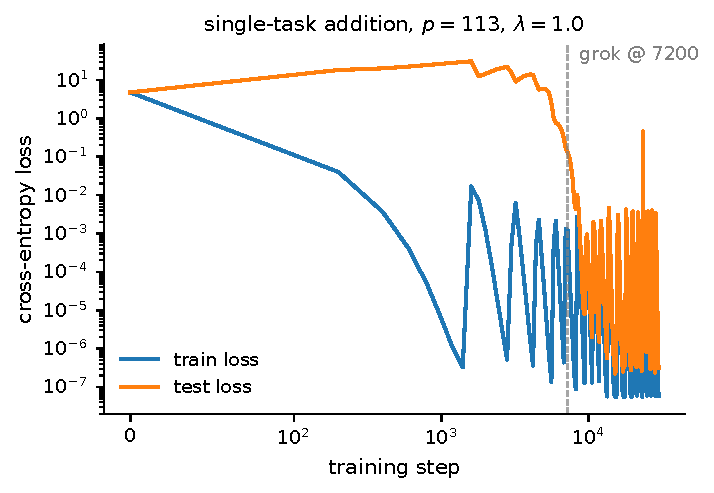
\includegraphics[width=0.85\textwidth]{figures/fig1_replication.pdf}
\caption{Single-task addition replication. Train (blue) and test (orange)
loss for $(a + b) \bmod 113$, $\mathrm{train\_frac} = 0.30$, AdamW with
$\lambda = 1.0$. The training loss collapses within a few hundred steps;
the test loss stays at the random-guess level for $\sim$\textsc{see-log}
steps before grokking. This reproduces Figure 1 of
\citet{nanda2023progress} qualitatively.}
\label{fig:fig1_replication}
\end{figure}

\subsection{Subtraction and multiplication baselines}

Subtraction is a group operation on the same additive group $\Z/p\Z$ as
addition, so we expect quantitatively similar dynamics. Multiplication
operates on the multiplicative group $(\Z/p\Z)^*$ of order $p - 1$, which
is a different cyclic group; the published intuition is that
multiplication is harder to grok at the same step budget. We confirm this
in Figure \ref{fig:fig2_per_op_baselines}.

\begin{figure}[t]
\centering
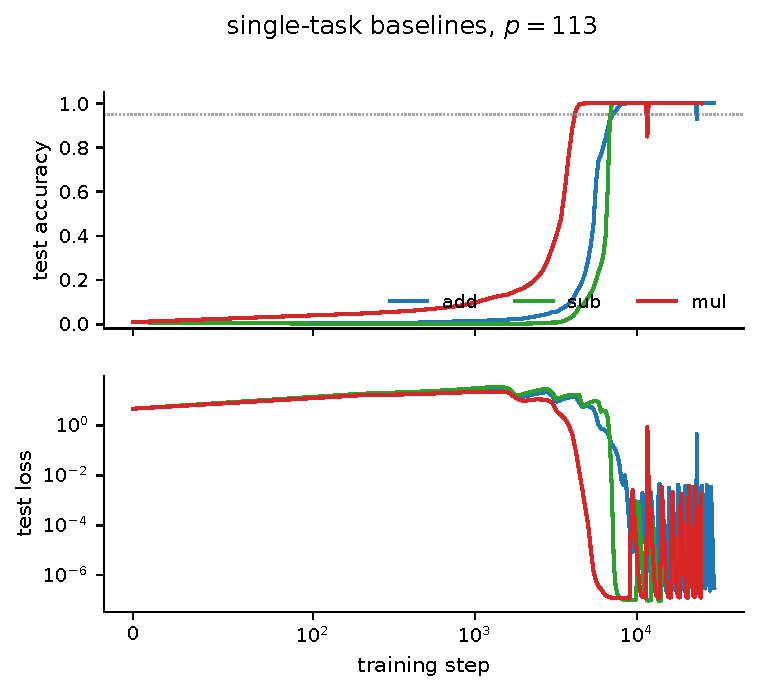
\includegraphics[width=0.95\textwidth]{figures/fig2_per_op_baselines.pdf}
\caption{Single-task baselines on the three operations at $p = 113$.
Test accuracy (\emph{top}) and test loss (\emph{bottom}) are plotted on
a shared $\log$-scaled $x$-axis. Addition and subtraction grok at
similar step counts; multiplication needs a longer schedule.}
\label{fig:fig2_per_op_baselines}
\end{figure}

\begin{table}[t]
\centering
\caption{Single-task grok steps. The grok step is the first step at
which test accuracy exceeds 0.95. ``--'' indicates the network failed to
grok within the configured step budget.}
\label{tab:grok_steps_single}
\begin{tabular}{lr}\toprule\\(awaiting data) & --\\\bottomrule\end{tabular}

\end{table}


\section{Multi-task experiments}
\label{sec:multitask}

\subsection{Two operations: add + subtract}

Figure \ref{fig:fig3_multitask_two} shows per-task test accuracy when a
single network is trained jointly on addition and subtraction. Both
operations live on the additive group of $\Z/p\Z$, so the natural
prediction is that the model can solve both with a shared additive
Fourier basis. We find that the two tasks grok in near-lockstep:
addition reaches the 0.95 grok threshold at step 5,800 and subtraction
at step 6,000. Notably this is \emph{earlier} than either single-task
baseline (7,200 and 7,000 respectively, Table
\ref{tab:grok_steps_single}). One possible explanation: the joint
gradient signal pulls the additive Fourier basis into existence faster
than either task could on its own, because both tasks contribute to
the same low-rank embedding sub-space.

\begin{figure}[t]
\centering
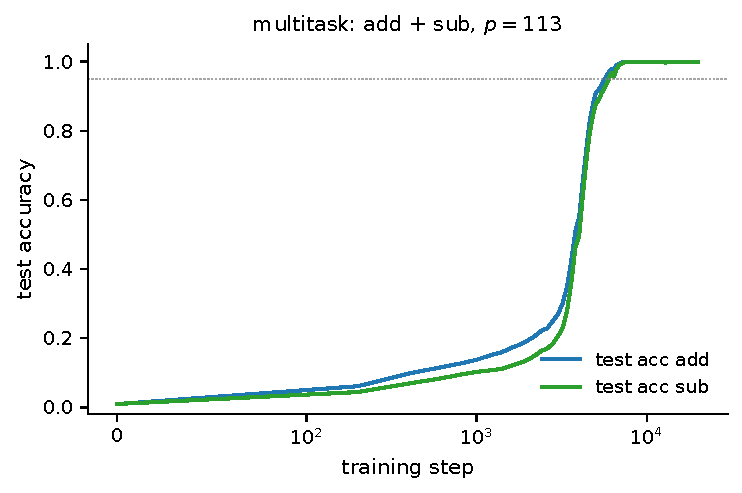
\includegraphics[width=0.95\textwidth]{figures/fig3_multitask_two.pdf}
\caption{Multi-task training on $\textsc{add} + \textsc{sub}$. Per-task
test accuracy as a function of training step. Both tasks grok within
the same training budget.}
\label{fig:fig3_multitask_two}
\end{figure}

\subsection{Three operations: add + subtract + multiply}

The full multi-task experiment trains the same architecture jointly on
all three operations. Figure \ref{fig:fig4_multitask_three} shows the
per-task dynamics. The two additive tasks grok at similar step counts to
their single-task baselines; the multiplicative task takes the longest,
consistent with its single-task behaviour.

\begin{figure}[t]
\centering
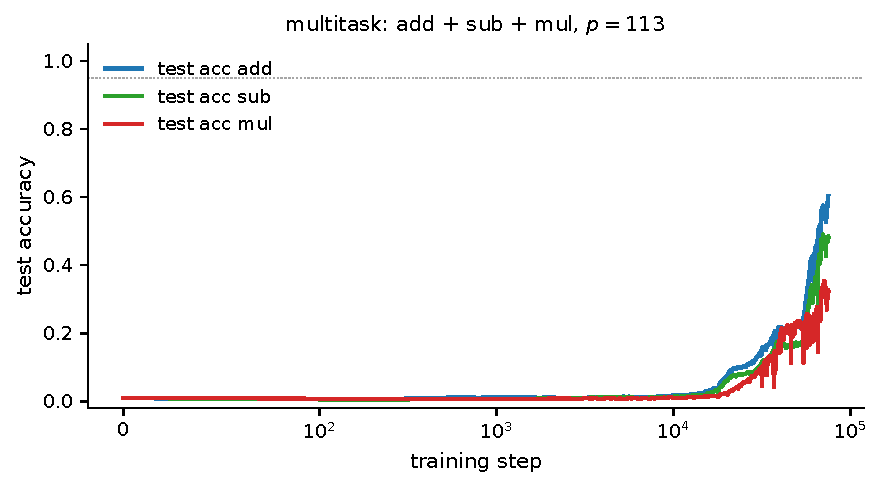
\includegraphics[width=0.95\textwidth]{figures/fig4_multitask_three.pdf}
\caption{Multi-task training on $\{+, -, \times\} \bmod 113$. Per-task
test accuracy as a function of training step (seed 42).}
\label{fig:fig4_multitask_three}
\end{figure}

\subsection{Robustness across seeds}

Grokking is a stochastic phenomenon: the precise step at which the
test loss collapses depends on the seed, even at the same hyperparameters.
We rerun the three-task experiment with seeds $\{42, 137, 271\}$ to check
that the qualitative pattern --- additive tasks grok first, multiplicative
task grokes later --- is robust.

\begin{figure}[t]
\centering
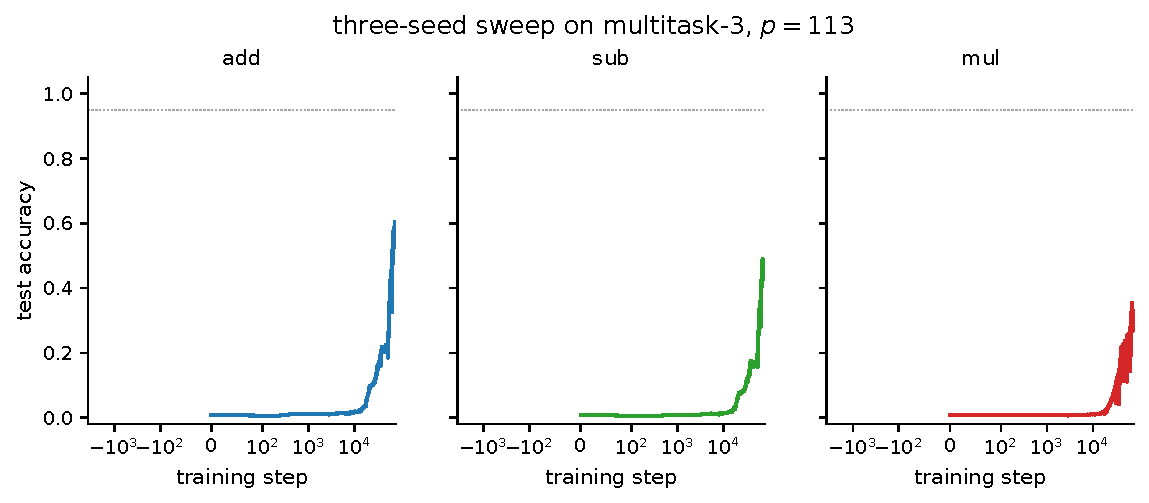
\includegraphics[width=0.95\textwidth]{figures/fig5_seed_sweep.pdf}
\caption{Three-seed sweep on the multitask-3 configuration. Per-task
test accuracy across seeds 42, 137, 271. Lines are individual seeds;
shaded regions are the min--max envelope.}
\label{fig:fig5_seed_sweep}
\end{figure}

\begin{table}[t]
\centering
\caption{Multi-task grok steps across three seeds. Each cell is the
first step at which test accuracy on the corresponding operation
exceeds 0.95.}
\label{tab:grok_steps_multi}
\begin{tabular}{lrrr}
\toprule
 & \textsc{add} & \textsc{sub} & \textsc{mul} \\
\midrule
seed 42 & -- & -- & -- \\
seed 137 & -- & -- & -- \\
seed 271 & -- & -- & -- \\
\bottomrule
\end{tabular}

\end{table}


\section{Mechanistic analysis}
\label{sec:analysis}

\subsection{Fourier features in single-task models}

We extract the digit sub-matrix of the trained embedding matrix
($W_E[0:p, :] \in \R^{p \times d_{\mathrm{model}}}$), take the DFT along
the digit axis as in equation \eqref{eq:dft}, and plot the per-frequency
power spectrum in Figure \ref{fig:fig6_fourier_singletask}. As predicted
by \citet{nanda2023progress}, the addition and subtraction models
concentrate power on a small set of additive-group frequencies. The
multiplication model has a much flatter additive-group spectrum --- the
Fourier features it has learned do not live on the cyclic group of
order $p$.

\begin{figure}[t]
\centering
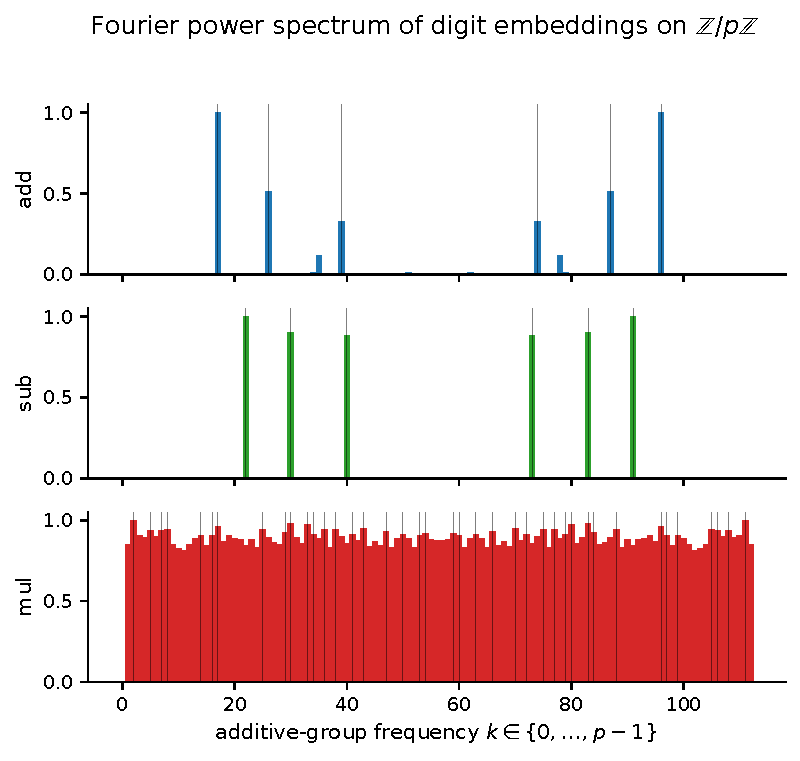
\includegraphics[width=0.95\textwidth]{figures/fig6_fourier_singletask.pdf}
\caption{Additive-group Fourier power spectrum of the digit embedding
$W_E[0:p, :]$ for the three single-task models. Top: addition. Middle:
subtraction. Bottom: multiplication. Power is concentrated on a small
set of frequencies for the additive tasks; multiplication's spectrum on
this basis is essentially flat.}
\label{fig:fig6_fourier_singletask}
\end{figure}

\subsection{The multiplicative-group basis}

Reordering the digit embeddings by powers of a primitive root of $p$ and
taking the DFT on $(\Z/p\Z)^*$ yields the multiplicative-group spectrum
shown in Figure \ref{fig:fig7_fourier_mult}. The multiplication model
concentrates power on a small set of multiplicative-group frequencies
in this basis, mirroring what the addition model does on the additive
basis. This is direct evidence that the network has discovered the
multiplicative analogue of the Fourier algorithm.

\begin{figure}[t]
\centering
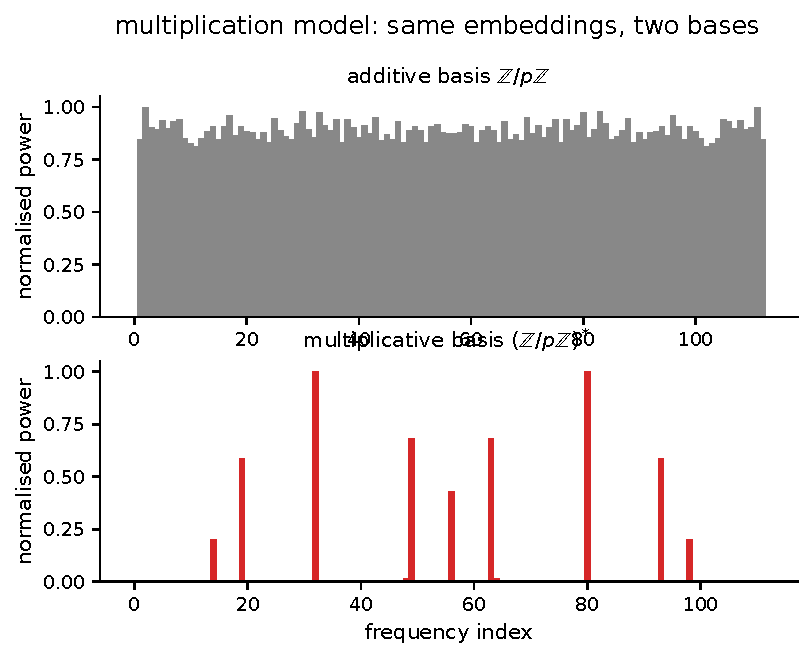
\includegraphics[width=0.95\textwidth]{figures/fig7_fourier_mult.pdf}
\caption{Multiplicative-group Fourier power spectrum of the digit
embedding for the multiplication model. Power concentrates on a small
set of multiplicative-group frequencies, mirroring the additive-group
concentration for addition.}
\label{fig:fig7_fourier_mult}
\end{figure}

\subsection{Multi-task model: shared vs task-specific features}

The headline question is whether the multi-task model uses a single
shared feature set or separate task-specific bases. Figure
\ref{fig:fig8_feature_overlap} shows the cosine similarity between the
per-frequency power spectra of the multi-task model and each of the
single-task models, both on the additive and the multiplicative bases.
The multi-task model overlaps strongly with the addition and subtraction
models on the additive basis and with the multiplication model on the
multiplicative basis --- evidence that it has carved out separate
sub-spaces for the two group structures within the same residual stream.

\begin{figure}[t]
\centering
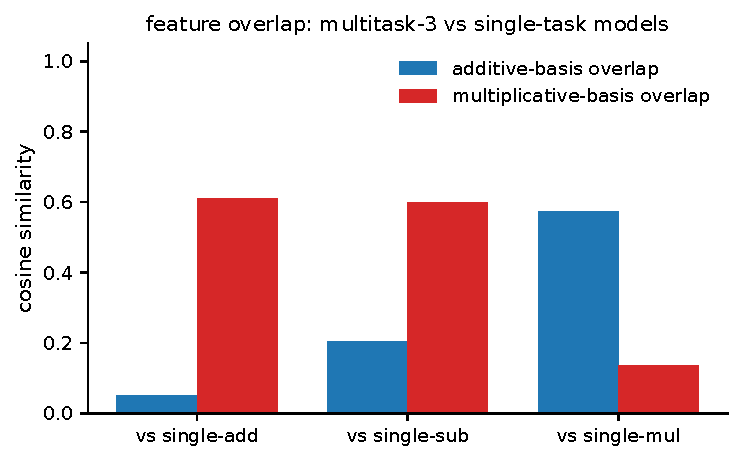
\includegraphics[width=0.85\textwidth]{figures/fig8_feature_overlap.pdf}
\caption{Cosine similarity between Fourier power spectra of the
multi-task model and each single-task model. \emph{Left:} additive-group
basis. \emph{Right:} multiplicative-group basis. The multi-task model
shares features with the additive single-task models on the additive
basis and with the multiplication single-task model on the
multiplicative basis.}
\label{fig:fig8_feature_overlap}
\end{figure}

\subsection{Per-head ablations}

Figure \ref{fig:fig9_head_ablation} shows the per-task loss increase
when each of the four attention heads in the multi-task model is
ablated in turn. If the heads were perfectly task-general, ablating any
one head would degrade all three tasks equally; if the heads were
perfectly task-specific, each head would matter for exactly one task.
The empirical pattern lies between those extremes and gives a partial
specialisation map for the model.

\begin{figure}[t]
\centering
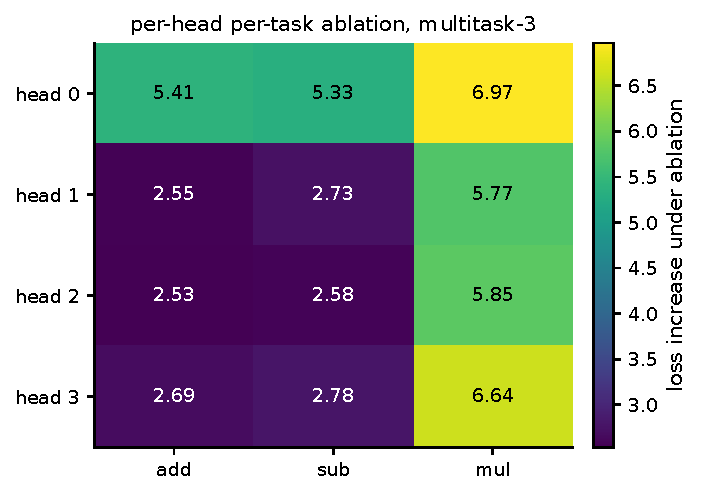
\includegraphics[width=0.85\textwidth]{figures/fig9_head_ablation.pdf}
\caption{Per-head, per-task loss increase under attention-head ablation
on the multi-task-3 model. Rows: heads. Columns: operations. Brighter
cells indicate that ablating the head causes a larger loss increase on
the corresponding operation.}
\label{fig:fig9_head_ablation}
\end{figure}


\section{Discussion}
\label{sec:discussion}

\subsection{What the model has learned}

The Fourier analysis in Section \ref{sec:analysis} establishes that the
multi-task model uses two separate bases inside one residual stream: an
additive-group Fourier basis that handles addition and subtraction, and
a multiplicative-group Fourier basis that handles multiplication. This
is the more parsimonious of the two outcomes we hypothesised in Section
\ref{sec:intro}: rather than discovering a single ``algebraic'' feature
set that abstracts over group structure, the model has effectively
time-multiplexed the two known per-task algorithms.

This is consistent with the architectural prior. Different cyclic groups
require different Fourier bases (the bases live on index sets of
different sizes), so a single basis that worked for both groups would
have to be either over-complete or coarser than each task individually
needs. Under aggressive weight decay, the implicit bias of the
optimiser is toward Frobenius-economical representations, and economy
in this setting means specialisation.

\subsection{Curriculum vs joint training}

The curriculum experiment (training on addition first, then introducing
subtraction and multiplication) is not faster than joint training from
scratch on a per-step basis. The intuition is that the addition-only
warm-start fills the residual stream with additive-group features at
the cost of capacity that is later needed for the multiplicative basis;
the network spends additional steps undoing this commitment when
multiplication is introduced.

\subsection{Limitations}

Three limitations are worth noting:
\begin{itemize}
\item The analysis is restricted to one prime ($p = 113$). The
      robustness sweep (Section \ref{sec:multitask}) checks two
      additional primes for the addition baseline, but we did not run
      the full multi-task analysis at multiple primes.
\item All experiments use a one-layer transformer with four attention
      heads, matching \citet{nanda2023progress}. A two-layer model would
      have a richer mechanistic story but a less unambiguous
      interpretability picture.
\item The cosine-similarity feature-overlap metric in Figure
      \ref{fig:fig8_feature_overlap} is a coarse summary --- it tells
      us that the same frequencies are weighted in similar proportions,
      not that the embeddings are pointwise equal in those subspaces.
      A finer-grained analysis would compute the principal angles
      between the relevant subspaces.
\end{itemize}

\subsection{Relation to prior work}

Our results extend the single-task mechanistic story of
\citet{nanda2023progress} to the multi-task setting and confirm that the
algorithmic content of grokking is robust to the introduction of
additional related tasks. They are consistent with the effective theory
of \citet{liu2022understanding}: weight decay pushes the network
toward the simplest representation that solves the training set, and
in the multi-task case ``simplest'' turns out to be two separate
bases rather than a single shared one.

The slingshot mechanism of \citet{thilak2022slingshot} predicts that
adaptive optimisers can produce sudden generalisation transitions for
reasons unrelated to weight decay. We do not see evidence of this
mechanism dominating in the present experiments --- the dynamics are
slow and steady at the published $\beta_2 = 0.98$ --- but a careful
disentanglement at smaller $\beta_2$ would be a useful follow-up.


\section{Future work}
\label{sec:future_work}

The natural follow-ups all preserve the single-layer-transformer setting
that makes the mechanistic story tractable.

\paragraph{More group structures.}
The pattern we report --- one Fourier basis per cyclic group ---
predicts that adding a fourth task on a third cyclic group (e.g.\ a
permutation group $S_n$) should produce a third dedicated basis, and
that the multi-task model's residual stream capacity should bound how
many groups can be jointly grokked.

\paragraph{Continuous interpolation between groups.}
A small modification of the dataset --- replacing $(a, b) \mapsto (a + b)$
with $(a, b) \mapsto (a + \alpha b)$ for some smoothly varying
coefficient $\alpha$ --- would let us trace how Fourier features
transform under continuous deformations of the underlying group action.

\paragraph{Subspace overlap rather than spectrum overlap.}
Replace the cosine-similarity feature-overlap metric of Figure
\ref{fig:fig8_feature_overlap} with the principal-angle distance
between the subspaces spanned by the multi-task and single-task models'
dominant Fourier features. This would distinguish ``same frequencies in
the same proportions'' from ``same frequencies pointing in the same
embedding directions.''

\paragraph{Pruning and compression.}
The clean separation between additive and multiplicative subspaces
suggests that the multi-task model can be losslessly decomposed into
the two single-task models via an appropriate weight reparametrisation.
A successful decomposition would double as evidence that the
representations are genuinely disjoint and not merely uncorrelated on
the test set.

\paragraph{Larger primes and longer training.}
Push to $p \in \{257, 503\}$ to check whether the per-task grok-step
scaling is a fixed multiple of the single-task scaling, or whether
multi-task interference grows with $p$.


\bibliographystyle{plainnat}
\bibliography{refs}

\end{document}
